\section{Grundlagen}
    \subsection{Limitationen}
        \begin{frame}{\secname: \subsecname}
            \begin{itemize}
                \item »Alle interessanten Fragen über das Verhalten eines Programms sind unentscheidbar.« (M. Schwartzbach)
                \item Saloppe Zusammenfassung des Satzes von Rice
                \item Annäherung an das korrekte Ergebnis ist weiterhin möglich
            \end{itemize}
        \end{frame}

    \subsection{Ansätze}
        \begin{frame}{\secname: \subsecname}
            \framesubtitle{Einfache Stringsuche/reguläre Ausdrücke}
            \begin{itemize}
                \item Wird sehr schnell sehr kompliziert:\\
                      \lstinline@mysql_query\\((["'])SELECT .+ FROM .+ WHERE .+(?:\\=|\\s+I?LIKE\\s+|<>|>=?|<=?).+\\1\\)@
            \end{itemize}
            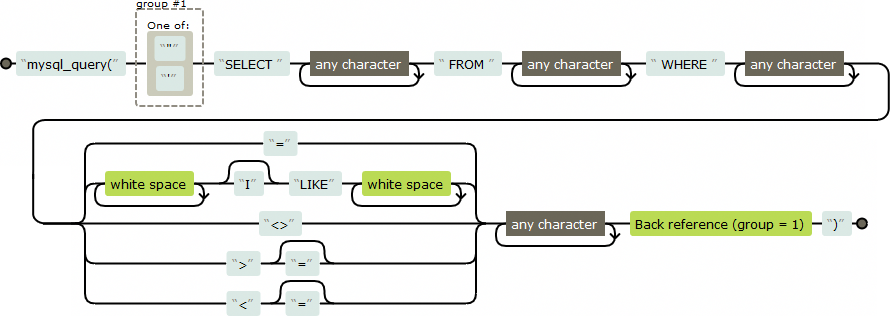
\includegraphics[keepaspectratio,height=\textheight,width=\columnwidth]{SQLi-RegEx.png}
        \end{frame}

        % \begin{frame}{\secname: \subsecname}
        %     \framesubtitle{Symbolische Ausführung}
        %     \begin{itemize}
        %         \item Programm wird simuliert
        %         \item Bedingungen werden mittels Constraint Solver getestet (SAT-Problem)
        %         \item Großes Problem: Pfadexplosion
        %         \item Erfordert exakte Definition des Programmablaufs
        %     \end{itemize}
        % \end{frame}

        \begin{frame}{\secname: \subsecname}
            \framesubtitle{Erstellung eines Parsers}
            \begin{itemize}
                \item Einfachere Abfragen als Stringsuche
                \item Keine Simulation des Laufzeitverhaltens
                \item[\textrightarrow] Kann unbekannte Bestandteile überspringen
                \item[\textrightarrow] Einfachere Erstellung eigener Sprachdefinitionen
                \item Für das Framework genutzter Ansatz
            \end{itemize}
        \end{frame}

    \subsection{Begriffe}
        \begin{frame}{\secname: \subsecname}
            \begin{itemize}
                \item Quelle (Source): Erzeugt benutzerdefinierte Eingaben
                \item Senke (Sink): Potentiell verwundbare Funktion
                \item Absicherung (Sanitizer): Sichert Eingaben für Senken ab
                \item Verschmutzung (Taint): Senke, die eine benutzerdefinierte Eingabe erhält
            \end{itemize}
        \end{frame}
